\documentclass[8pt]{beamer}
\usetheme{default} % Very simple theme
\usecolortheme{dove} % Minimalist grayscale colors
\setbeamertemplate{navigation symbols}{} % Remove navigation bar

% Define brand-like colors
\definecolor{myblue}{RGB}{0, 102, 204}    % Blue for standard blocks
\definecolor{mygreen}{RGB}{0, 153, 0}     % Green for example blocks
\definecolor{myred}{RGB}{204, 0, 0}       % Red for alert blocks
\definecolor{myorange}{RGB}{255, 128, 0} % For \emph

% Accent color for titles, bullets, etc.
\setbeamercolor{structure}{fg=myblue}

% Block colors
\setbeamercolor{block title}{bg=myblue, fg=white}
\setbeamercolor{block body}{bg=blue!5, fg=black}

\setbeamercolor{exampleblock title}{bg=mygreen, fg=white}
\setbeamercolor{exampleblock body}{bg=green!5, fg=black}

\setbeamercolor{alertblock title}{bg=myred, fg=white}
\setbeamercolor{alertblock body}{bg=red!5, fg=black}
\setbeamercolor{alerted text}{fg=myred}

% Optional: color for \example text
\setbeamercolor{example text}{fg=mygreen}

% Custom emph (orange text instead of italic)
\let\oldemph\emph
\renewcommand{\emph}[1]{\textcolor{myorange}{#1}}


\usepackage{graphicx} % Package for images
\usepackage{amsmath} % Package for images
\graphicspath{{figs/}} % Path to your figures directory
\usepackage{array}  % For better column spacing
\usepackage{caption} % Required for \captionof

% Title Information
\title{STOCHASTIC METHODS IN WATER RESOURCES}
\vspace{25pt}
\subtitle{Unit 1: Introduction to probability and statistics \\ Lecture 4a: Model estimation and testing}
\author{Luis Alejandro Morales, Ph.D.}
\institute{Universidad Nacional de Colombia \\ Department of Civil and Agriculture Engineering} %// }
%\date{\today}

\begin{document}

% Title Slide
\begin{frame}
    \titlepage
\end{frame}

%-------
% From Kotte
\section{Generalities}
\begin{frame}{Generalities}
    \begin{itemize}
        \item Statistical inference deals with  statistical estimations based on a \emph{sample} from the \emph{population}.
        \item Some definitions:
            \begin{itemize}
                \item \alert{Population}: consist of all possible observations of a process (e.g. air temperature at certain location). Some of the observations in the in the population may not have any physical sense, perhabs, due to sensor errors. 
                \item \alert{Sample}: is a subset of the population (e.g. instantaneous daily streamflow for a certain period in a station). A \emph{random sample} is thus a sample that is representative of the population.
                \item \alert{Random variables}: is a \emph{real-valued function} defined on a \emph{sample space}. Wheather a random variable is \emph{discrete} or \emph{continuous} depends on how the sample space is defined. 
                \item \alert{Statistic}: is a function of the observations that is quantifiable and does not contain any unknown parameter. Note that a \emph{statistic} is also a random variable that provides an \emph{estimation}.
                \item \alert{Estimator}: is the method or rule of estimation. For instance, the \emph{sample mean} $\bar{X}$ is a point estimator of the \emph{population mean} $\mu$. 
                \item \alert{Estimate}: is the value yielded by the estimator. 
                 \end{itemize}
             \item Suppose that the population of variable $X$ follows a \emph{Normal distribution} and the distribution parameters $\theta$ are unknown. Thus, a random sample of $X$ of size $n$.
             \item Parameters $\theta$ can be described by a number or a range; this last include an uncertainty. 
    \end{itemize}
\end{frame}

%-------
% From Kotte
\section{Properties of estimators}
\begin{frame}{Properties of estimators}
    
    \begin{block}{Unbiasedness}
        Given a sample of observations of a random variable $X$, $X_1, X_2, \cdots, X_n$, the objective is to estimate the value of the parameter $\theta$, which is also a random variable. The idea is to seek for a \emph{estimator} of  $\theta$ that get as closest as possible to the \emph{true value}. This estimator will produce statistics that are distributed following a certain \emph{pdf}. Following this, a \alert{point estimator $\hat{\theta}$}  is an \alert{unbiased estimator} of the population parameter $\theta$ if $E[\hat{\theta}] = \theta$. If the estimator is biased, the $\text{bias} = E[\hat{\theta}] - \theta$.
    \end{block}
    
    \begin{exampleblock}{Mean of the sample mean}
        Let us show that the sample mean $\bar{X}$ is an unbiased estimator of $\mu$. If $\bar{X} = \frac{1}{n} \left( X_1 + X_2 + \cdots + X_n \right) $, then $E[\bar{X}] = \frac{1}{n} nE[X_i] = \frac{1}{n} (n \mu) = \mu$. 
    \end{exampleblock}
    Note that many estimator are biased and methods such as \emph{jackknife} and \emph{bootstrap} are used to reduce the bias. Ideal estimator must also have the following properties. 
    \begin{block}{Consistency}
        An estimator $\hat{\theta}_n$, based on a sample size $n$, is a \alert{consistent} estimator of $\theta$ if for any positive number $\varepsilon$ $\lim_{n\rightarrow \infty} Pr[ | \hat{\theta}_n - \theta | \leq \varepsilon ] = 1$
    \end{block}

    \begin{block}{Minimum variance}
        A part for looking for an unbiased estimator, it is also desirable to seek for an \alert{minimum variance estimator}. The \emph{minimum variance unbiased estimator} is the estimator with the smallest variance out of all unbiased estimator
    \end{block}


\end{frame}
    

\begin{frame}{Properties of estimators}
\begin{block}{Efficiency}

    \vspace{-5pt}
    \alert{Efficiency} is the relative measure of the variance of the sampling distribution, with the efficiency increasing as the variance decrease. In terms of the \emph{mean square error (mse)} an estimator with the minimum $mse$ among all possible unbiased estimators is called and \alert{efficient estimator}. If $A$ is an estimator of $\theta$, the $mse$ is:
    \begin{align*}
        E\left[(A-\theta)^2\right] &= E\left[ \left( \left(A - E[A] \right) - \left( \theta - E[A] \right) \right)^2 \right]  \\
                                                                                                                                  &= E[ (A - E[A])^2 ] + (\theta - E[A])^2 \\
                                                                                                                                  &= Var[A] - bias^2
    \end{align*}
    The $mse$ of an estimator can be used as a relative measure of efficiency when comparing two or more estimator. 
    \end{block}

    \vspace{-7pt}
\begin{block}{Sufficiency}
    So far, properties such as unbiasedness, consistency and the minimum $mse$ are key to select the most suitable estimators. Thus, a \alert{sufficient estimator} provides as much information as possible about a sample of observations of a random variable $X$. Let a sample $X_1, X_2, \cdots, X_n$ be drawn randomly from population having probability distribution with unknown parameters $\theta$. Thus, the statistic $T = f(X_1, X_2, \cdots, X_n)$ is said to be sufficient to estimate $\theta$ if the distribution of $X_1, X_2, \cdots, X_n$ conditional to the statistics $T$ is independent of $\theta$.    
    \end{block}
    \vspace{-9pt}
    \begin{exampleblock}{Median and mean}
        The \emph{median}, taken as a measure of mean density or central tendency, does not contain all the information in a sample. The median is the middle value of the sample; if any other value is changed the mean changes but the median is unaltered.
    \end{exampleblock}

\end{frame}

%-------
% From Kotte
\section{Estimation of confidence intervals}
\begin{frame}{Estimation of confidence intervals}
    The uncertainty of point estimates can be quantified by the relative variances or mean square errors of the estimators. Because of this uncertainty, the next step of inference is \alert{interval estimation}. Two numbers, say, $a$ and $b$, that are expected to include within their range an unknown parameter $\theta$ in a specified percentage of cases after repeated experimentation under identical conditions. That is, in place of one statistic that estimates $\theta$, we find a range specified by two statistics, which includes it at a given level of probability. The end points $a$ and $b$ of this range are known as \alert{confidence limits}, and the interval $(a, b)$ is known as the \alert{confidence interval}. We do not have the precision as for a point estimator but we have confidence (without absolute certainty) that the assertion is right.

\begin{block}{Confidence interval estimation of the mean when the standard deviation is known}
    Let $C_l$ and $C_u$ be the \emph{lower} and \emph{upper} confidence limits that include an unknown but invariable parameter $\theta$. Although there is some uncertainty associated with this statement, we will be right in a proportion, say, $1 – \alpha$, of the samples taken from the same population, on average, when we make the assertion that the given interval includes $\theta$. Thus we can say, by adopting the long-run frequency interpretation of probability,
\[
    Pr[C_l  \leq \theta \leq C_u ] = 1 - \alpha
\]
where $\theta$ is a constant, but the estimator $\hat{\theta}$  and the confident limits $C_l$ and $C_u$ are random variables. Recall that examples of $\hat{\theta}$ are $\bar{X}$ and $\bar{S}^2$. The probability $(1 – \alpha)$ is known as the \emph{confidence level} or \emph{confidence coefficient}. It often takes values such as 0.99, 0.95, and 0.90. The confidence limits $C_l$ and $C_u$ depend on the sampling distribution of $\theta$. The standard deviation of the statistic $\hat{\theta}$ called its \emph{standard error}.

    \end{block}
\end{frame}

\begin{frame}{Estimation of confidence intervals}
\begin{block}{Confidence interval estimation of the mean when the standard deviation is known}
    In some situations, we may require \emph{one-sided confidence limits}. The \emph{lower and upper one-sided confidence limits} are specified, respectively, by
    \[
        Pr[C_l \leq \theta] = 1 - \alpha \quad \text{for } 0 < \alpha < 1
    \]
    and

    \[
        Pr[\theta \leq C_u] = 1 - \alpha \quad \text{for } 0 < \alpha < 1
    \]
\end{block}

\begin{minipage}[t]{0.54\textwidth}
   \vspace{0pt} % prevent extra spacing at top
    Let $\bar{X}$ be the mean of a random sample of size $n$ drawn from a population with known standard deviation $\sigma$. The $100(1 – \alpha)$ percent central two-sided confidence interval for the population mean $\mu$ is $\left( \bar{X} - z_{\alpha/2} \frac{\sigma}{\sqrt{n}}, \bar{X} + z_{\alpha/2} \frac{\sigma}{\sqrt{n}} \right)$, where $z_{\alpha/2}$ is a standard normal variate that is exceeded with probability $\alpha/2$, $Z = \frac{\bar{X}- \mu}{\sigma/\sqrt{n}} \quad N \sim (0,1)$. The one-sided upper and lower $100(1 – \alpha)$ percent confidence limits for the population mean $\mu$ are, $\bar{X} + z_{\alpha} \frac{\sigma}{\sqrt{n}} $ and $\bar{X} - z_{\alpha} \frac{\sigma}{\sqrt{n}} $, respectively. 
\end{minipage}
%\hfill
\begin{minipage}[t]{0.44\textwidth}
   \vspace{0pt} % prevent extra spacing at top
    \centering
    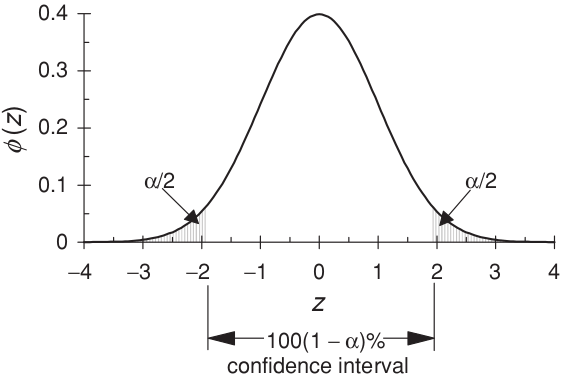
\includegraphics[width=\textwidth]{fi531.png}
\end{minipage}

\end{frame}


\begin{frame}{Estimation of confidence intervals}
    \begin{block}{Confidence interval estimation of the mean when the standard deviation is unknown}
        Quite often in practice the mean and standard deviation are both unknown. Under such conditions we must modify our approach. We assume normality of the variate $X$ as before, but the consequences of a \emph{nonnormal distribution} are minor for small to moderate departures from normality, if the sample size is large, say, $n > 30$. In this situation we apply the \emph{Student’s t distribution}.
\end{block}
\end{frame}

\end{document}
